%\documentclass[draft]{ws-procs9x6}
\documentclass{llncs}
\usepackage{comment}
\usepackage{subfigure}
\usepackage{color}
\usepackage{epsfig}
\usepackage{times}
\usepackage{url}
\begin{document}

\title{Improving local multiple alignment of interspersed DNA repeats with gapped extension}

\author{Todd J. Treangen\inst{1}$^\dag$, Aaron E. Darling\inst{2}$^\dag$, Mark A. Ragan\inst{2},Xavier Messeguer\inst{1}}
%
\authorrunning{<Treangen> et al.}   % abbreviated author list (for running head)
%
\institute{ Dept. of Computer Science, Technical Univ. of Catalonia, Barcelona, Spain\\
\email{treangen@lsi.upc.edu},\\
\and Institute for Molecular Bioscience, The University of Queensland, Brisbane, Australia\\
\email{a.darling@imb.uq.edu.au},\\
 }

\maketitle
{\center \scriptsize $^\dag$ These authors contributed equally to this work \\}

\begin{abstract}
The identification of homologous DNA is a fundamental building block
of comparative genomic and molecular evolution studies. To date,
pairwise local sequence alignment methods have been the prevailing
technique to identify homologous nucleotides. However, existing
methods that identify and align all homologous nucleotides in one or
more genomes have suffered poor scalability and limited accuracy. We
propose a novel method that couples a gapped extension heuristic with
a previously described efficient filtration method for local multiple
alignment.  During gapped extension, we use the MUSCLE implementation
of progressive multiple alignment with iterative refinement.  The
resulting gapped extensions potentially contain alignments of
unrelated sequence.  We detect and
remove such undesirable alignments using a hidden Markov model to
predict the posterior probability of homology. The HMM
emission frequencies for nucleotide substitutions can be derived from
any strand/species symmetric nucleotide substitution matrix, and we
have developed a method to adapt an arbitrary substitution matrix
(i.e. HOXD) to organisms with different G+C content. We evaluate the
performance of our method and previous approaches on a hybrid dataset
of real genomic DNA with simulated interspersed repeats.  Our method
outperforms existing methods in terms of sensitivity,
positive predictive value, and localizing boundaries of homology.  The
described methods have been implemented in the free, open-source
\texttt{procrastAligner} software, available from: \\
\url{http://alggen.lsi.upc.es/recerca/align/procrastination}
\end{abstract}


%\keywords{sequence alignment, local multiple alignment, interspersed repeats, gapped extension, hidden Markov model}

\section{Introduction}
The importance of accurate homology identification to comparative
genomics can not be overestimated\cite{Kumar07}. To date, pairwise
local sequence alignment
methods such as BLAST\cite{ref-blastz,ref-ssearch,ref-pattern} have been the
prevailing technique to identify homologous nucleotides.  When more
than two copies of a homologous sequence element are present in the
data, pairwise homology detection methods generate a listing of all
possible pairs of homologous elements in the form of pairwise local
alignments.  Apart from the obvious inefficiency of considering all
pairwise homology relationships, a collection of pairwise alignments
is not ideal because they are rarely amenable to comparative genomic
and phylogenetic analysis without further processing into a multiple
alignment.

Local pairwise alignments can be merged to create a multiple alignment
by a variety of
methods\cite{ref-tba,ref-aba,ref-dialign,ref-related1}. Such methods
commonly assume that pairwise homology relationships are transitive,
such that if nucleotide $a$ is homologous to nucleotide $b$, and $b$
is to $c$, then $a$ must also be homologous to $c$.  Thus, in order to
merge pairwise alignments, such methods must tackle the challenging
problem of resolving inconsistent transitive homology relationships.
Multiple alignment has been demonstrated to be more accurate than
pairwise alignment, especially when dealing with a large number of
divergent sequences\cite{ref-mlagan,ref-aubergene}.  As the number of
homologous sequences grows, we might expect that the number of
inconsistent relationships in a collection of pairwise alignments
would grow quadratically, whereas a direct multiple alignment method
would provide an increasingly accurate alignment.  Moreover, highly
repetitive regions in the input sequences can cause serious efficiency
problems for pairwise methods, as they create $O(r^{2})$ pairwise
alignments in the presence of a repeat with $r$ copies.  Mammalian Alu
repeats and IS elements in microbes are two common examples of the
overwhelming abundance of repetitive sequence in whole genomes.

Local multiple alignment has the inherent potential to avoid pitfalls
associated with pairwise alignment. Although optimal multiple
alignment under the SP objective function remains
intractable\cite{ref-wangjiang}, progressive alignment heuristics
offer excellent speed and accuracy\cite{ref-clustalw,ref-tcoffee}
especially when combined with tree-independent iterative
refinement\cite{ref-muscle}, or probabilistic consistency
measures\cite{ref-probcons}. Rather than merging pairwise alignments,
why not exploit years of research into multiple alignment heuristics
by directly constructing a multiple alignment? We thus present a novel
heuristic for directly computing local multiple alignments via gapped
extension of chained seed matches.

\section{A heuristic for gapped extension of multiple alignments}
Our method for computing local multiple alignments exploits the MUSCLE
multiple alignment algorithm to compute gapped extensions of ungapped
multi-match seeds (see Figure~\ref{fig-main}). Gapped alignments arise
when extending seeds to fully capture surrounding sequence
homology. Our method assumes that a fixed number of nucleotides
flanking a seed match are likely to be homologous and computes a
global multiple alignment on the flanking region.  Our assumption of
flanking homology often proves to be erroneous and results in an
alignment of unrelated sequences.  In the context of \textit{local}
multiple alignment, the fundamental problem with such an approach is
that current methods for progressive alignment with iterative
refinement compute \textit{global} alignments, i.e. they implicitly
assume that input sequences are homologous over their entire length.
To resolve the problem, we employ a hidden Markov model which detects
unrelated regions embedded in the global multiple alignment.
Unrelated regions are then removed from the alignment and the
local-multiple alignment is trimmed to reflect the updated boundaries
of homology.

Our method for local multiple alignment, depicted for an example sequence in
Figure~\ref{fig-main}, has seven primary steps: (1) identify
multi-match seeds in the input sequence, (2) chain individual
seeds, (3) multiple alignment of regions between chained seeds, (4)
gapped extension of seed chains (5) detection of unrelated regions
using a hidden Markov model, (6) application of transitive homology
relationships, and (7) unalignment of any unrelated sequence to
produce final local multiple alignment.  Steps 1-2 have been previously
described\cite{ref-procrast}, while steps 3-7 represent a new contribution
and are the subject of the present manuscript. Steps 2-7 are applied
repeatedly to seeds identified in step 1 to produce local multiple
alignments of all homologous nucleotides in the input sequence.

\begin{figure}[p]
\begin{center}
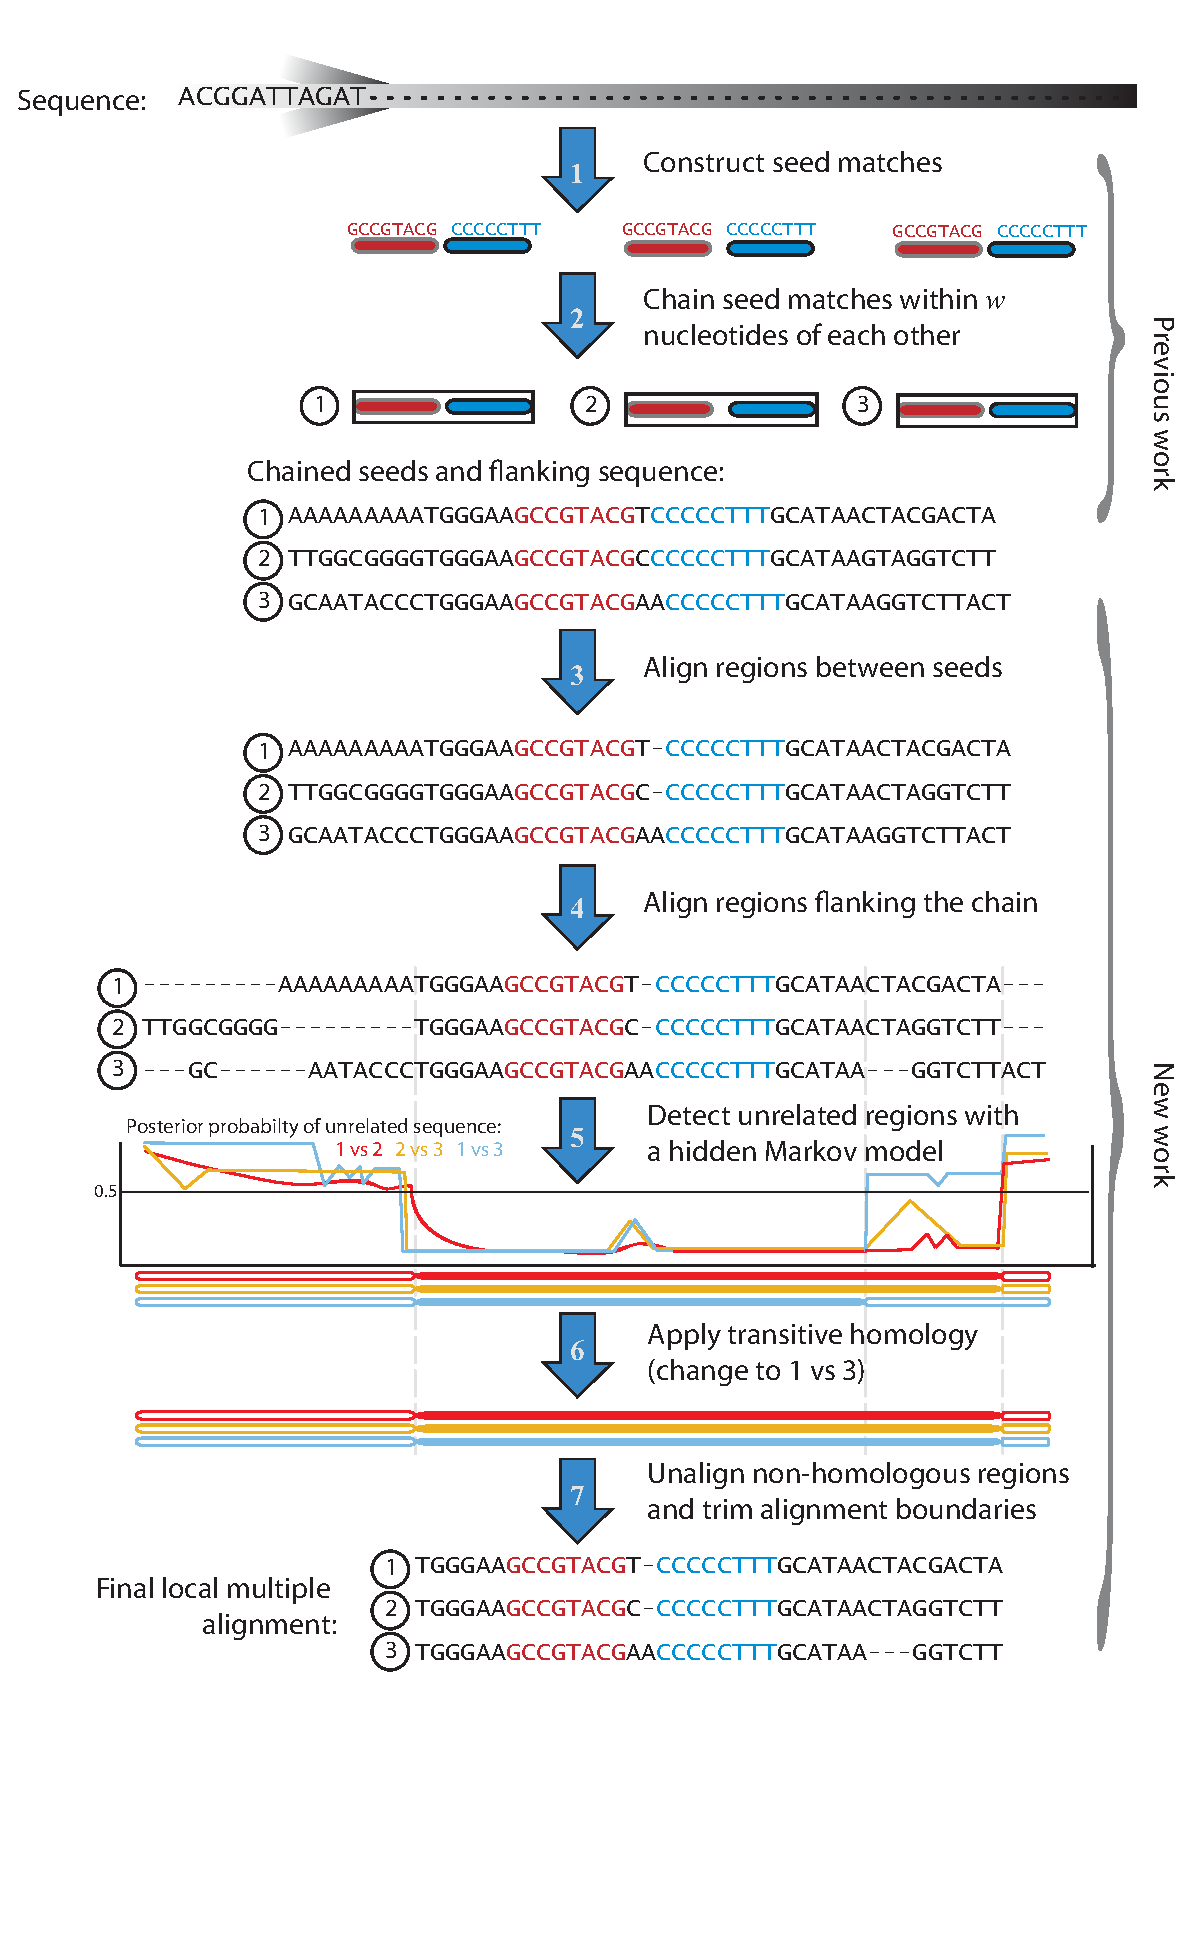
\epsfig{file=./figures/extension.eps,width=4.1in}
%\subfigure[Visual representation of our algorithm]{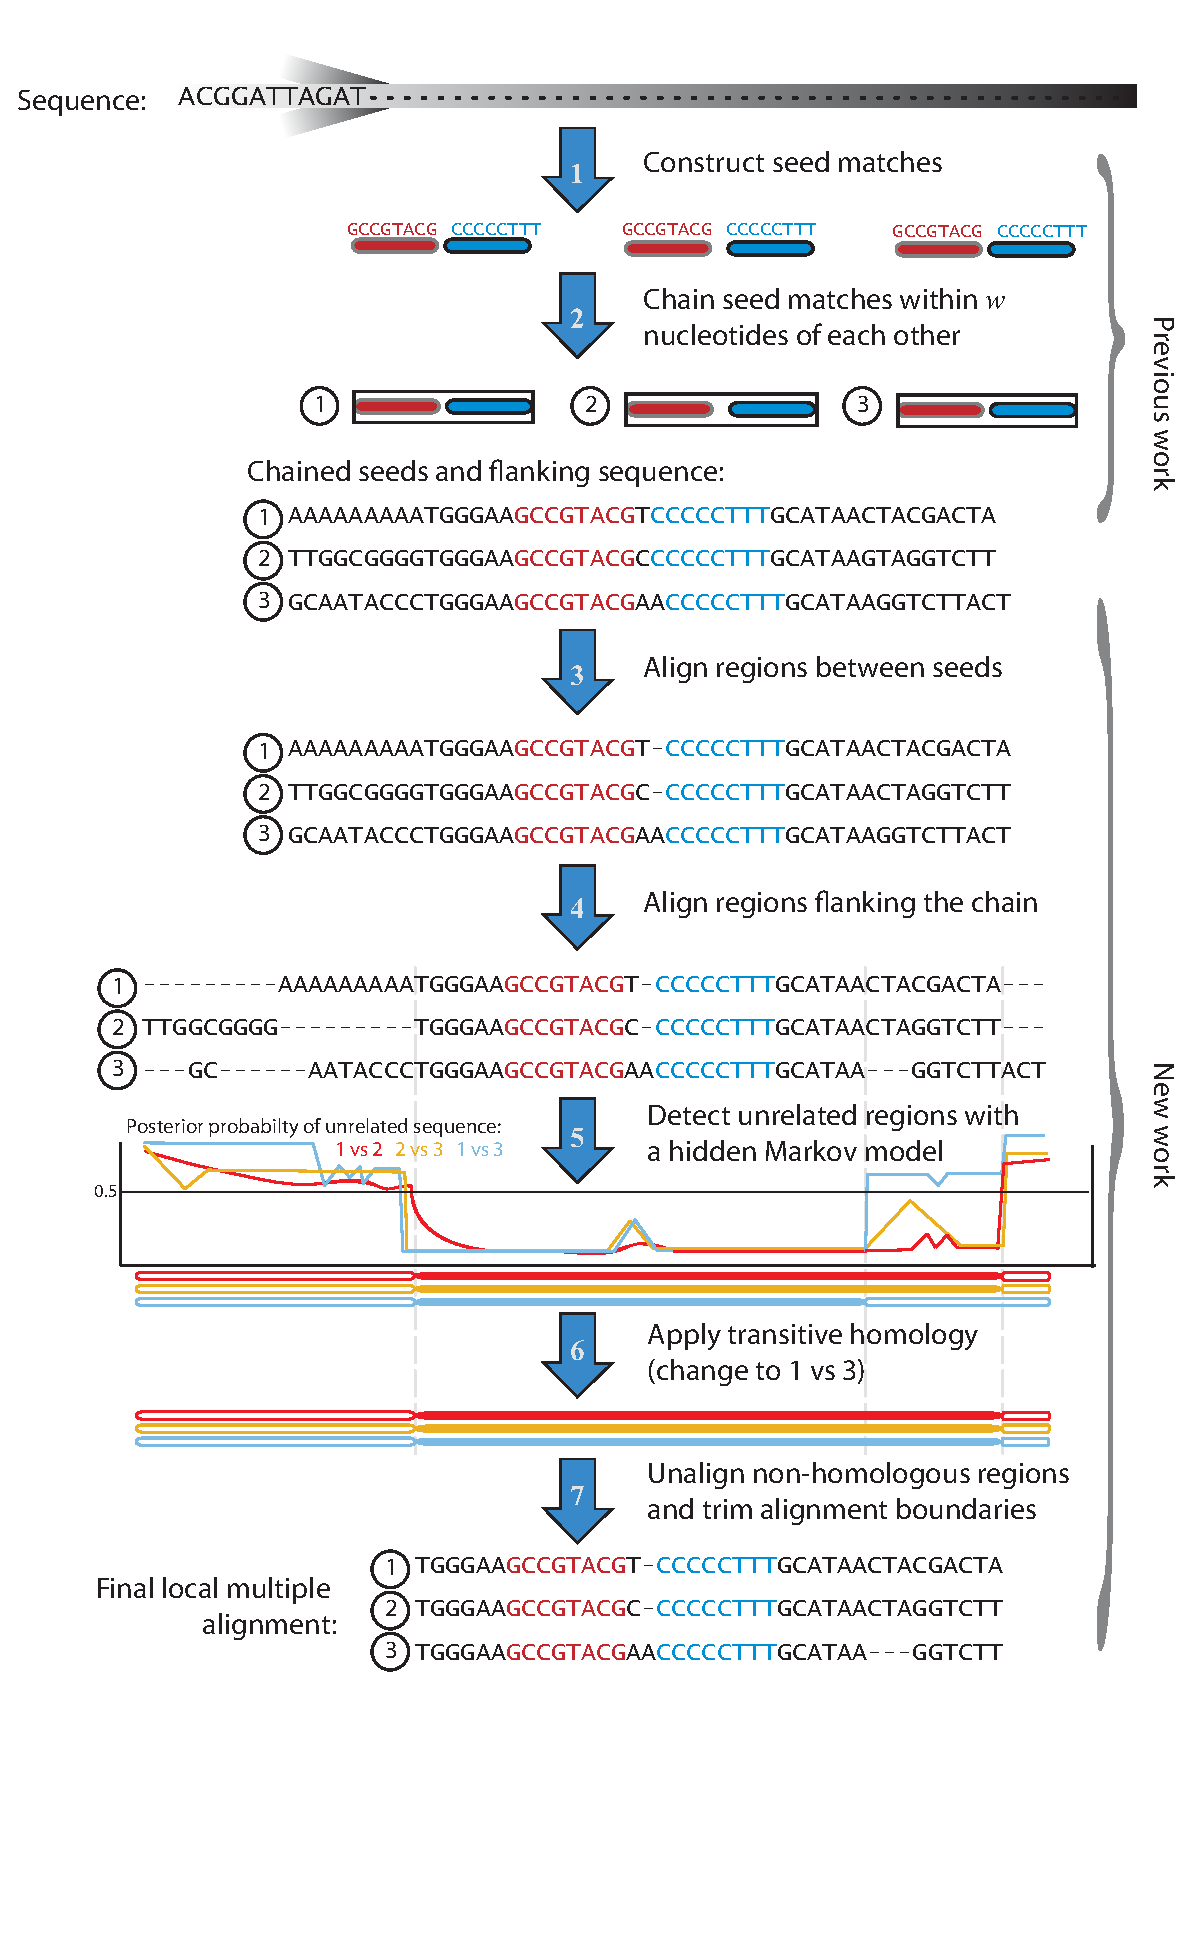
\epsfig{file=./figures/extension.eps,width=3.0in}}
%\subfigure[Flowchart of the algorithmic process ]{ 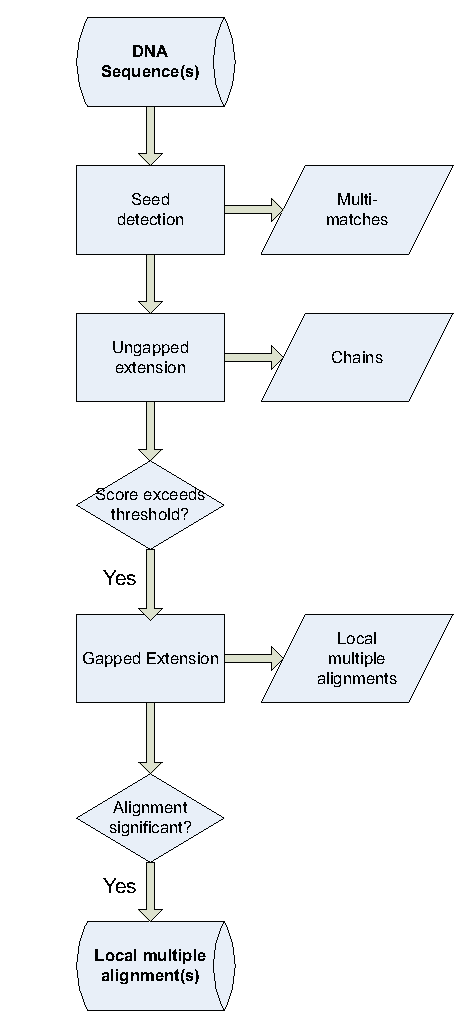
\epsfig{file=./figures/flowchart.eps,width=1.7in}}
\end{center}
\vspace{-1.6cm}
\caption{Overview of the method, starting with an input sequence and ending
with a set of local multiple alignments. First we (1) detect
multi-matches in the input sequence(s) using palindromic spaced seeds,
then we perform (2) chaining and extension of all multi-matches within
$w$ nt of each other.  In the present example, one chain exists and
contains two matches each with three match components labeled 1, 2,
and 3.  We then perform gapped alignment of the region between chained
matches (3).  In step (4), we perform a gapped extension by computing
a global multiple alignment on the regions to the left and right of
each chain component.  The resulting alignment may contain unrelated
sequence, so in step (5) we apply a hidden Markov model to detect
poorly aligned regions indicative of unrelated sequence.  Step (6)
computes transitive homology relationships to ensure a consistent
alignment and aid detection of divergent homologous sequences.
Finally, in step (7) we unalign regions found to be non-homologous.
If we find after step (2) that the alignment boundaries have been
extended, we return to step (4) for another round of chaining.}
\label{fig-main}
\end{figure}

\subsection{Chaining multi-matches from the input sequence}
Given a sequence $\mathcal{S}=s_1, s_2,\dots, s_N$ of length $N$
defined over an alphabet $\{A,C,G,T\}$, our goal is to identify all
significant local multiple alignments on subsequences of
$\mathcal{S}$. Our method first extracts candidate ungapped
alignments, or multi-matches, among subsequences in $\mathcal{S}$,
denoted as $\mathbf{M}$. To extract multi-matches from the input
sequence, we utilize a palindromic spaced seed pattern\cite{ref-zhang}, which is
analyzed at each position in the input sequence.  Previously we have
demonstrated that palindromic spaced seeds offer good efficiency and
reasonable sensitivity on a variety of input
sequences\cite{ref-procrast}.  We refer the number of matching regions
in $\mathcal{S}$ by a given match $M_i \in \mathbf{M}$ as the
\textit{multiplicity} of $M_i$, denoted as $|M_i|$. We refer to each
matching region of $M_i$ as a \textit{component} of $M_i$. Our
algorithm has an important limitation on the matches in $\mathbf{M}$:
no two matches $M_i$ and $M_j$ may have the same left-end coordinate,
except for the identity case when $i=j$.  This constraint has been
referred to by others as \textit{consistency} and
\textit{transitivity}\cite{ref-transitivity} of matches.

Once a list of multi-matches has been generated, we employ an
efficient chaining and filtration algorithm to identify overlapping
and nested chains of multi-matches\cite{ref-procrast}. In order to
chain process each region of sequence $\mathcal{O}(1)$ times, matches
are prioritized for chaining in order of decreasing multiplicity.  Our
method chains seed multi-matches of the same multiplicity $M_{i}$
occurring within $w$ characters of each other.  When a multi-match can
no longer be chained without including a gap larger than $w$
characters, neighboring \textit{subset} matches within $w$ characters
are identified. Each neighboring subset match is then \textit{linked}
to the chained match. We refer to the chained match as a
\textit{superset} match. Rather than immediately extend the subset
match(es), we \textit{procrastinate} and extend the subset match later
when it has the highest multiplicity of any match waiting to be
extended. When chaining a match with a linked superset, we immediately
include the entire region covered by the linked superset match and
thus eliminate the need to re-examine sequence already covered by a
previously chained match.

\subsection{Gapped extension of high-scoring chains}
After chaining a multi-match $M_i$, we perform gapped alignment on all
collinear regions located between two adjacent components to generate
unextended local multiple alignments. We first evaluate the chain to
decide whether expending computational resources on gapped extension
will be worthwhile. We can require that two or more seeds be present
in the chain and use lower seed weights ($k$), a technique which has
previously been proven
successful\cite{ref-blastz,ref-gappedblast,ref-blat}.  To perform a
gapped extension in each direction, we use MUSCLE to align a fixed
number of nucleotides ($l$) to the left and right of the current local
multiple alignment.  Small values of $l$ restrict the alignment search
space, while larger values require more computation but are
potentially more sensitive.  We have empirically determined that
setting $l$ based on multiplicity ($l = 70e^{-0.01*|M_{i}|}$) offers a
good tradeoff between speed and sensitivity.  The resulting extension
window is small for high multiplicity chains ($|M_{i}|\geq 30$),
keeping the alignment search space tractable.
%\begin{equation}
% \max(w, \sqrt{(\max(150^{2}-(2*|M_{i}|)^{2},0)}));
%\end{equation}

\subsubsection{Identifying unrelated regions}
\begin{figure}[t]
\centering 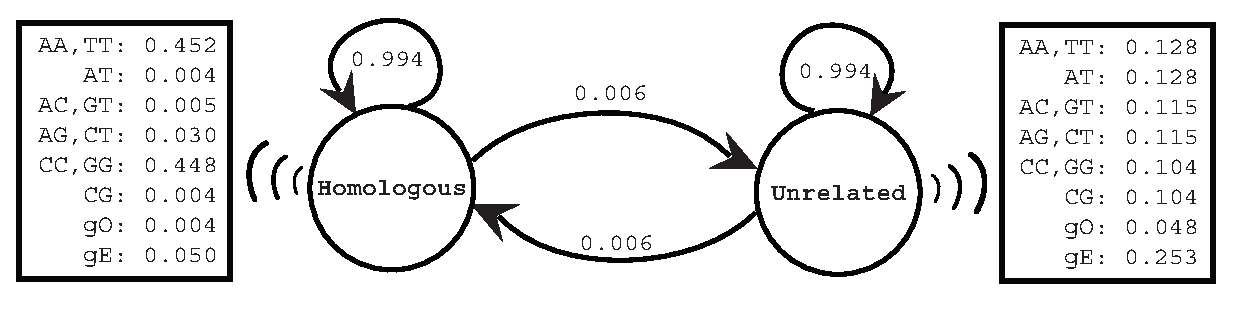
\epsfig{file=./figures/hmm.eps,width=4.6in}
\caption{\textbf{Hidden Markov model used to detect pairwise alignments of unrelated
sequence.} \scriptsize The HMM has states which model alignment columns containing
homologous and unrelated sequence. Emission probabilities are extracted from the HOXD substitution matrix and correspond to alignment
columns, for example \texttt{AA} indicates A aligned to A.  gO
indicates gap-open and gE gap extend. Alignment columns are treated as
strand-symmetric, so that AC also indicates CA and the reverse
complements TG and GT.  The emission probabilities are adjusted to the GC content of the input genome
as described in the test.  The values shown here correspond to a 47.5\% GC genome.}
\label{fig-hmm}\vspace{-0.2cm}
\end{figure}
The MUSCLE alignment software dutifully reports the highest scoring
global multiple alignment of input sequences, regardless of whether
they are related by common ancestry. As a consequence of the gapped
extension process, it is likely that our method forcibly aligns unrelated
sequence. We have configured a hidden Markov model (Figure
~\ref{fig-hmm}) to detect alignments of unrelated sequence. The HMM
consists of two hidden states, Homologous and Unrelated. The
observable states are the pairwise alignment columns, which are all
possible pairs in $\texttt{{\{A,G,C,T,-\}}}$ with strand and species
symmetry, i.e. \texttt{AG=GA=TC=CT}. The emission probabilities for
each possible pair of aligned nucleotides were extracted from the HOXD
substitution matrix presented by Chiaromonte \textit{et al}\cite{hoxd}.
We solved for the emission frequencies in the
homologous and unrelated state using the same equation used in to
calculate the values of the HOXD substitution matrix on 47.5\%G+C
content sequence\cite{hoxd}:
\begin{equation}
s(x,y)= \log_{2}{\Bigg(\frac{p(x,y)}{q_{1}(x)q_{2}(y)}\Bigg)}
\end{equation}
{w}here $p(x,y)$ is the fraction of the observed aligned pairs of
nucleotides $x$ and $y$ in the training set used and $q_{1}(x)$ and
$q_{2}(y)$ denote the background frequencies of $x$ and $y$,
respectively. Chiaramonte \textit{et al.} scaled the resulting
$s(x,y)$ values by $\psi=32.5421$ so the largest was 100,
with the rest rounded to the nearest integer.

HMM probabilities can be derived using any strand/species symmetric nucleotide substitution matrix,
but any particular matrix makes specific assumptions about divergence time, mutation pressures,
and sequence composition of the aligned sequences.
Genomes can range in G+C content from 30-75\%, and at the extremes,
a substitution matrix derived on 47.5\% GC sequence (such as HOXD) does not
perform well.  We have thus developed a method to adapt HMM emission
frequencies derived from an arbitrary substitution matrix
to organisms with different G+C content.  Emission
probabilities in the Unrelated state can be directly adapted to the
background nucleotide distribution as follows:
\begin{center}
$U_{AA}=U_{AT}=U_{TA}=U_{TT}=(\frac{f_{AT}}{2})(\frac{f_{AT}}{2})$
$U_{CC}=U_{CG}=U_{GC}=U_{GG}=(\frac{f_{GC}}{2})(\frac{f_{GC}}{2})$
$U_{AC}=U_{AG}=U_{TC}=U_{AG}=(\frac{f_{AT}}{2})(\frac{f_{GC}}{2})$
$U_{CA}=U_{CT}=U_{GA}=U_{GT}=(\frac{f_{GC}}{2})(\frac{f_{AT}}{2})$
\end{center}
where the notation $U_{XY}$ indicates the probability of observing nucleotide X aligned to
nucleotide Y in Unrelated sequence.  $f_{AT}$ is the fraction of nucleotides which are A/T and
$f_{GC}$ is the fraction of GC in the input genome.  Note that $f_{AT}=1-f_{GC}$.


\textbf{FIXME: NEW DESCRIPTION ON HOW WE ADAPT EMISSION PROBABILITIES... IS THIS OK?}
Adapting emission probabilities in the Homologous state is a bit more
involved, as we need to separate the substitution probability,
$Q(x,y)$, from the background frequency, $\pi(x)$.  To perform this
decomposition we need to divide the original $p(x,y)$ (fraction of the
observed aligned pairs of nucleotides $x$ and $y$ in the training set)
by $\pi(x)$ from the HOXD data (i.e. $\pi$=.475 for G/C and .525 for
A/T) and then multiply by the $\pi(x)$ for the genome under
consideration. A problem arises in the A/T$->$G/C mutations, however,
since A/T has a different $\pi(x)$ than G/C and we don't know the
direction of time, the time of divergence and the ancestral
state. Thus, we make an assumption that the probability of either
nucleotide at the root node is equal to their background frequencies
in the sequence. Using this assumption we are able to adapt the
Homologous state emission probabilities as follows:
\begin{center}
$H^{'}_{AG}=H_{AG}$, \ \ \ $H^{'}_{AC}=H_{AC}$ \\
$H^{'}_{AA}=(\frac{f^{'}_{AT}}{f_{AT}})H_{AA}$, \ \ \ \
$H^{'}_{AT}=(\frac{f^{'}_{AT}}{f_{AT}})H_{AT}$\\
$H^{'}_{CC}=(\frac{f^{'}_{GC}}{f_{GC}})H_{CC}$, \ \ \ \
$H^{'}_{CG}=(\frac{f^{'}_{GC}}{f_{GC}})H_{CG}$\\
\end{center}
where $H^{'}_{xy}$ are the $H_{xy}$ values adapted to the input genome's G+C content.

%more description need here? to supplemental material?
\begin{comment}
Taking  A G pair for example, we have
pi_A * exp{Q(A,G)t} + pi_G*exp{Q(G,A)t}  but since the substitution
process is reversible, Q(A,G)=Q(G,A) and so we're left with
(pi_A+pi_G)*exp{Q(A,G)t}.  So the thing to do here is divide by the
original pi_A+pi_G and multiply by the new pi_A+pi_G.  For the HOXD the
original pi_A+pi_G is 0.525/2 + 0.475/2 = 0.2625+0.2375 = 0.5.  And
indeed, by definition, the new pi_A+pi_G is also 0.5!  So we don't have
to do anything with those values.

I suppose a similar problem arises in the A->T mutations (also T->A, G-
>C, C->G).  for those we're looking at pi_A * exp{Q(A,T)t} + pi_T*exp{Q
(T,A)t}.  which reduces to (pi_A+pi_T)*exp{Q(A,T)t}.  Where pi_A+pi_T =
0.525 in the original HOXD data, and so we will want to compute it for
the new data and adjust emissions accordingly (by dividing old and
multiplying new, pre-gap-normalization.
\end{comment}

Emission frequencies for nucleotide substitutions can be derived from
any strand/species symmetric nucleotide substitution matrix, but gap-open
and extend frequencies can not.  To empirically estimate values
for the unrelated state we aligned a 10-kb, 48\%~G+C content region
taken from \emph{E. coli} CFT073 (Accession AF447814.1, coordinates
37,300-38,300) with an unrelated sequence.  We generated an unrelated
sequence with identical nucleotide composition by reversing the
extracted sequence without complementation.  We then forced an
alignment with MUSCLE and counted the number of gap-open and gap-extend
columns in the alignment of unrelated sequences.  Gap-open and
extend frequencies for the homologous state were estimated by
constructing an alignment of 10kb of orthologous sequence shared among
a pair of divergent organisms.  We aligned the 48\%G+C segment between
genes \textit{fruR} and \textit{secA} from \textit{E. coli} K12
(Accession U00096.21) and \emph{Y. pestis} CO92 (Accession
AL590842.1). We add the empirically derived gap-open and extend
frequencies for each state and normalize the emission frequencies to a
probability distribution.  The resulting emission probabilities are
reported in Figure~\ref{fig-hmm}. Using the empirically derived transition and emission probabilities,
we apply the posterior HMM decoder implemented in Gerton Lunter's
HMMoC software\cite{Lunter2007} to compute the posterior probability that
each alignment column represents homologous sequence.  Columns with a
p.p. below 0.5 are considered to be unrelated.  We then apply the
transitive homology principle to our predictions, resulting in a final
set of consistent homology predictions.  See Figure~\ref{fig-main},
steps 5 and 6 for an example. We trim the alignment to exclude all
columns beyond the Homologous state. If the original boundaries were
improved, we trigger another round of chaining (and consequently
another round of extension) in the same direction.
When gapped extension fails to improve boundaries
in one direction, extension in the other direction is attempted until
no further extension is possible.


\section{Results}
\begin{figure}[t]
\centering 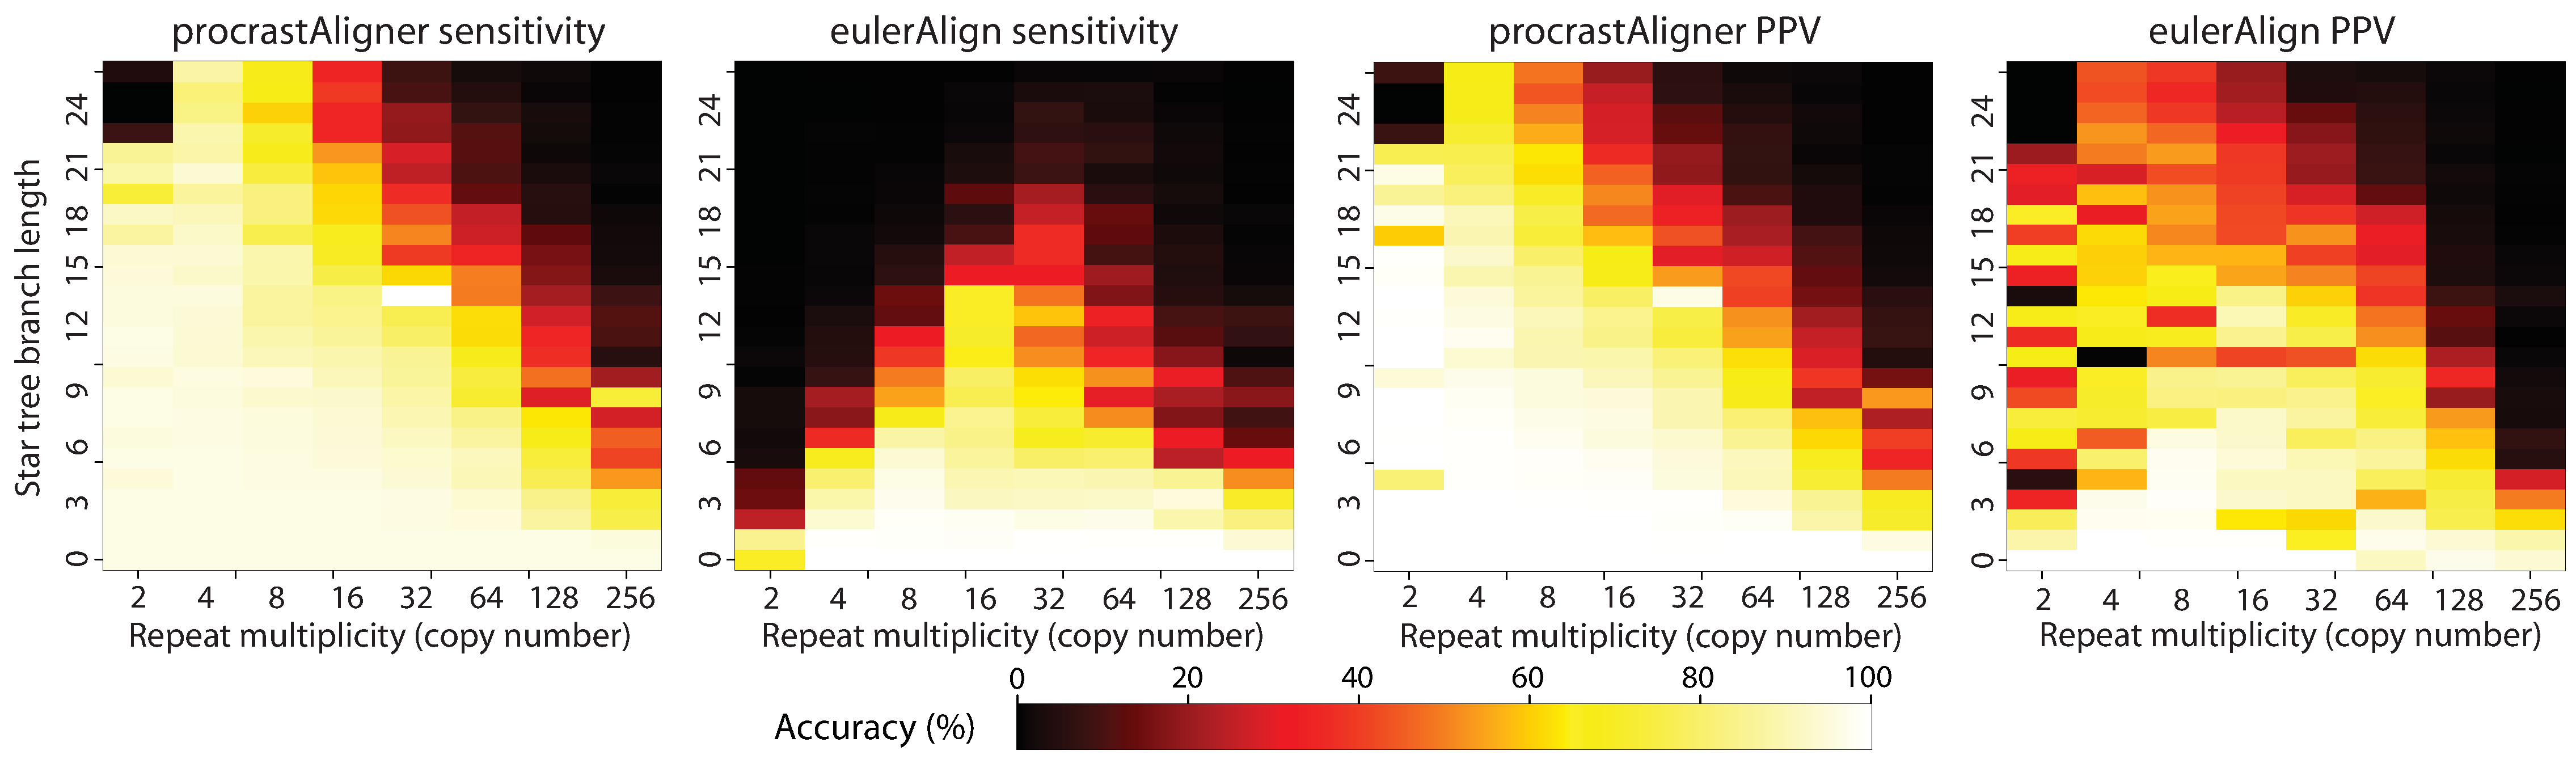
\epsfig{file=./figures/repeat_accuracy_new.eps,width=4.6in}
\caption{\textbf{Accuracy recovering simulated repeat families planted in the
\textit{Mycoplasma genitalium} genome}.  \scriptsize Sum-of-pairs nucleotide
sensitivity and positive predictive value (PPV) of \texttt{procrastAligner} and \texttt{eulerAlign} were measured for 200
combinations of branch length and multiplicity.  Three replicates of
each simulation were performed and average accuracy values are shown
here.  White points indicate perfect alignment of the simulated repeat
family.  Black points indicate the program completely failed to
recover any portion of the repeat family.  Mutations per site can be
calculated by multiplying branch length by the fixed substitution rate
of 0.09, and indel rate of 0.01.  For example, at branch length 20
there are 1.8 substitutions per site and 0.2 indels per site.  From
the figure, it is apparent that \texttt{procrastAligner} performs better
at higher mutation rates and multiplicities than \texttt{eulerAlign}.}
\label{fig-results}\vspace{-0.2cm}
\end{figure}

We have previously demonstrated the sensitivity of our chaining method
in finding Alu repeats in the human
genome\cite{ref-procrast}. Figure~\ref{fig-align} shows part of a
local multiple alignment of one such Alu family as generated with
\texttt{procrastAligner}. To highlight the benefits of our proposed
heuristic for gapped extension, we compare ~\texttt{procrastAligner}'s
performance to the Eulerian path method for local multiple alignment
as implemented by \texttt{eulerAlign}\cite{ref-related1}. The Eulerian
path method uses a \textit{de Bruijn} graph for filtration, and goes
beyond filtration to compute gapped alignments using banded dynamic
programming.  To our knowledge, \texttt{procrastAligner} and
\texttt{eulerAlign} represent the only two automated methods to
construct local multiple alignments directly from genomic DNA.

\subsection{Simulating interspersed repeats}
We evaluate accuracy of each method when aligning simulated repeat
families that have been inserted into the complete genome of
\emph{Mycoplasma genitalium}. The \emph{M. genitalium} genome has been recognized
as complex and repeat-rich, presenting a biologically
relevant and challenging example to evaluate alignment
methods\cite{ref-mycoplasma}. We simulated repeat families of 8
different multiplicities ranging between 2 and 256 ($x$-axis in
Figure~\ref{fig-results}).  Each repeat copy has an average length
based on its family's multiplicity
($length=\frac{7680}{multiplicity}$), thus high copy-number repeats
are short.  Evolution of repeat families was simulated as a marked
Poisson process on a star tree
topology.  The branch lengths were varied between 0 and 24 ($y$-axis
in Figure~\ref{fig-results}), with the nucleotide substitution rate
fixed at 0.09 per unit time, and the indel rate fixed at 0.01 per
unit time.  Rate heterogeneity among sites was modeled with a gamma
distribution ($\theta = 1.0, k = 0.5$).  Indel size was
Poisson distributed with intensity 3, and insertions and deletions
were taken to be equally likely.  Each family's ancestral
sequence was randomly generated using nucleotide frequencies equal to
the composition of \emph{Mycoplasma genitalium}
($A=0.34,T=0.34,G=0.16,C=0.16$). Insertion sites for repeat copies
were chosen uniformly at random in the 580kb \textit{M. genitalium} genome,
allowing tandem repeats but prohibiting mosaic repeats.

\subsection{Alignment accuracy metrics}
\label{sec:metrics}
We used each program to find local multiple alignments in each of the
200 modified \emph{M. genitalium} genomes and recorded alignment
accuracy as follows. We calculated sum-of-pairs nucleotide sensitivity
as $\frac{\mathrm{TP}}{\mathrm{TP} + \mathrm{FN}}$, where
$\mathrm{TP}$ is the number of aligned nucleotide pairs in the
program's output which are also aligned in the simulated repeat
family.  $\mathrm{FN}$ is the number of aligned nucleotide pairs in
the simulated repeat family which are missing from the program's
output.  This sensitivity measure is identical to the sum-of-pairs
accuracy defined by BaliBASE\cite{ref-balibase}.  We calculate the
positive predictive value (PPV) as $\frac{\mathrm{TP}}{\mathrm{TP} +
\mathrm{FP}}$, where $\mathrm{TP}$ is defined as above, and
$\mathrm{FP}$ is the total number of nucleotide pairs from the
program's output where one of the nucleotides are part of the
simulated repeat family and the other nucleotide was incorrectly
aligned.

We also quantify the ability of each aligner to accurately predict the
boundaries of the interspersed repeats.  For a given pair of repeat components, we calculate accuracy by
by recording the number of nucleotides between the true boundary and the predicted boundary
on both the right and left sides of the repeat.  Thus, over-extension gets a positive score, while underextension
yields a negative score and perfect boundaries receive a 0 score. See Figure~\ref{fig-overunder} for
further details on boundary under/overpredictions.

\begin{figure}[t]
\centering
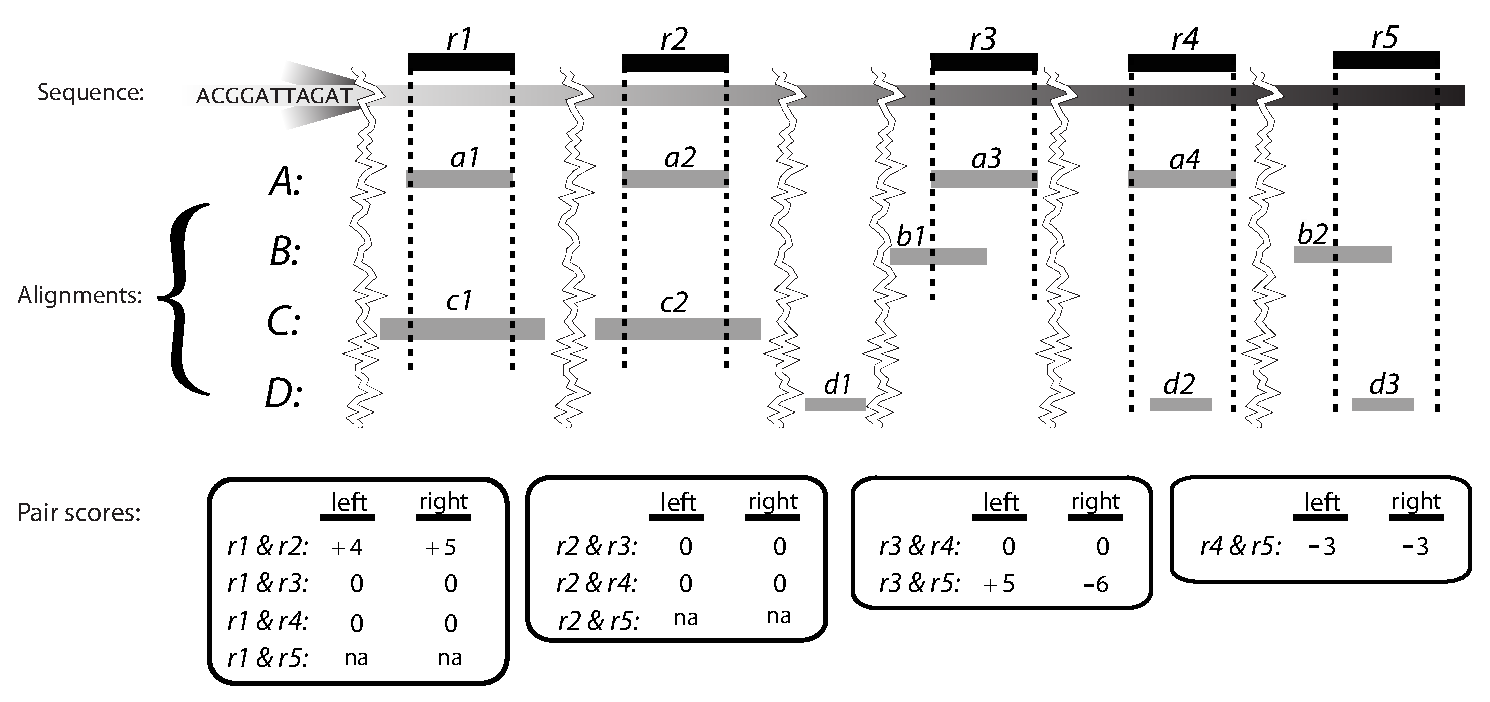
\epsfig{file=./figures/boundary_scores.eps,width=4.6in}
\caption{\textbf{Boundary accuracy metric}. \scriptsize We define our boundary accuracy metric to be a sum-of-pairs score by comparing the boundaries of all \emph{r} components of the inserted repeat \emph{R}. For any pair of components, $\emph{r}_{i}$ and $\emph{r}_{j}$, we take the maximum boundaries proposed by all local multiple alignments output using each program. The figure shows a multiplicity five interspersed repeat \emph{R} and four local multiple alignments, \emph{A, B, C, D}, containing the predicted boundaries for each component \emph{r} of \emph{R}. The vertical jagged lines represent breaks in otherwise contiguous sequence. There are four cases we need to consider for each component pair; each of these cases are diagrammed in the above figure: (1) \emph{Correct prediction}. Local multiple alignment {\emph{A}} correctly identifies the true right and/or left boundaries for repeat components: \emph{r1}, \emph{r2}, \emph{r3} and \emph{r4}. (2) \emph{Under \& overprediction}. Local multiple alignment \emph{B} overlaps repeat components \emph{r3} and \emph{r5}, and as a result, simultaneously under and overpredicts the true boundaries of this component of interspersed repeat. (3) \emph{Overprediction}. Local multiple alignment \emph{C} overpredicts the true boundaries of components \emph{r1} and \emph{r2} of the interspersed repeat. (D) \emph{Underprediction}. Local multiple alignment \emph{D} underpredicts the true boundaries of components \emph{r4} and \emph{r5}.
We also list the resulting component pair scores by taking the maximum boundaries between any two components contained in the same local multiple alignment. Underprediction is penalized by recording a negative penalty for the difference between the true left/right end boundaries, overprediction is penalized by recording a positive penalty of the difference, and correct boundary prediction is not penalized (penalty=0). Component pairs that are not aligned in any of the reported local multiple alignments are not scored, indicated by \emph{na}. Using our scoring metric, the average absolute distance from the true boundary is 1.50 (left side) \& 1.75 (right side).  }
\label{fig-overunder}
\end{figure}

\subsection{Accuracy when aligning interspersed repeats}
We applied \texttt{procrastAligner} and \texttt{eulerAlign} to the
hybrid simulated/real dataset.  Parameters used for each program were
configured to optimize each program's chance of accurately aligning
each pattern. \texttt{procrastAligner} was configured using \texttt{--z=15 --w=20}, and \texttt{eulerAlign} with \texttt{-k 15 -l -i 1000 -v}.
Simulations for each of the 200 combinations of branch length and
multiplicity were replicated three times and alignments generated in
parallel on a 156 node compute cluster.  Results of the experiments
are reported in Figure~\ref{fig-results} and
Figure~\ref{fig-boundary}. Figure~\ref{fig-results} illustrates the
sensitivity and PPV of \texttt{procrastAligner} and
\texttt{eulerAlign} on datasets ranging from 0 substitutions and
indels per site to 2.16 substitutions and 0.24 indels per site (branch length 24).  As
mutation rates and repeat multiplicity increase the alignment accuracy
decreases for both methods, with accuracy of \texttt{eulerAlign}
decreasing faster than \texttt{procrastAligner}.  Surprisingly, \texttt{eulerAlign}
often fails to align low multiplicity repeats, even when mutation rates are low.
Manual experimentation with \texttt{eulerAligner} parameters -v (tolerance for mismatches), -k (seed k-mer size) and -i (number of iterations) settings up to 10,000 failed to improve its performance on low-multiplicity repeats.
We conjecture that \texttt{procrastAligner}'s overall improved accuracy largely derives
from its use of spaced seed patterns\cite{ref-procrast} and tolerance
of gaps. The Eulerian path method requires exactly matching $k$-mers
to seed gapped alignment extensions.

In addition to sensitivity and PPV benchmarks, we also assess how well
each aligner recovers the true boundaries of interspersed
repeats.  Figure~\ref{fig-boundary} illustrates the ability of each
program to accurately localize the known boundaries of the simulated interspersed
repeats. From the figure, it is apparent that on average \texttt{procrastAligner} predicts
the exact repeat boundary for all studied combinations of branch length (repeat degeneracy)
and multiplicity (repeat copy number).  Moreover, the standard error in \texttt{procrastAligner}'s
boundary predictions is typically very low, within 4 nucleotides.  \texttt{eulerAlign}, on the other hand,
exhibits erratic behavior.  For low multiplicity repeats it has a strong tendency to
underpredict the repeat boundary.  At high multiplicities ($\geq32$) \texttt{eulerAlign} tends to
slightly overpredict the boundaries, by including flanking unrelated sequence in the alignment of
the interspersed repeat.

\begin{figure}[t!]
\centering
\subfigure[]{
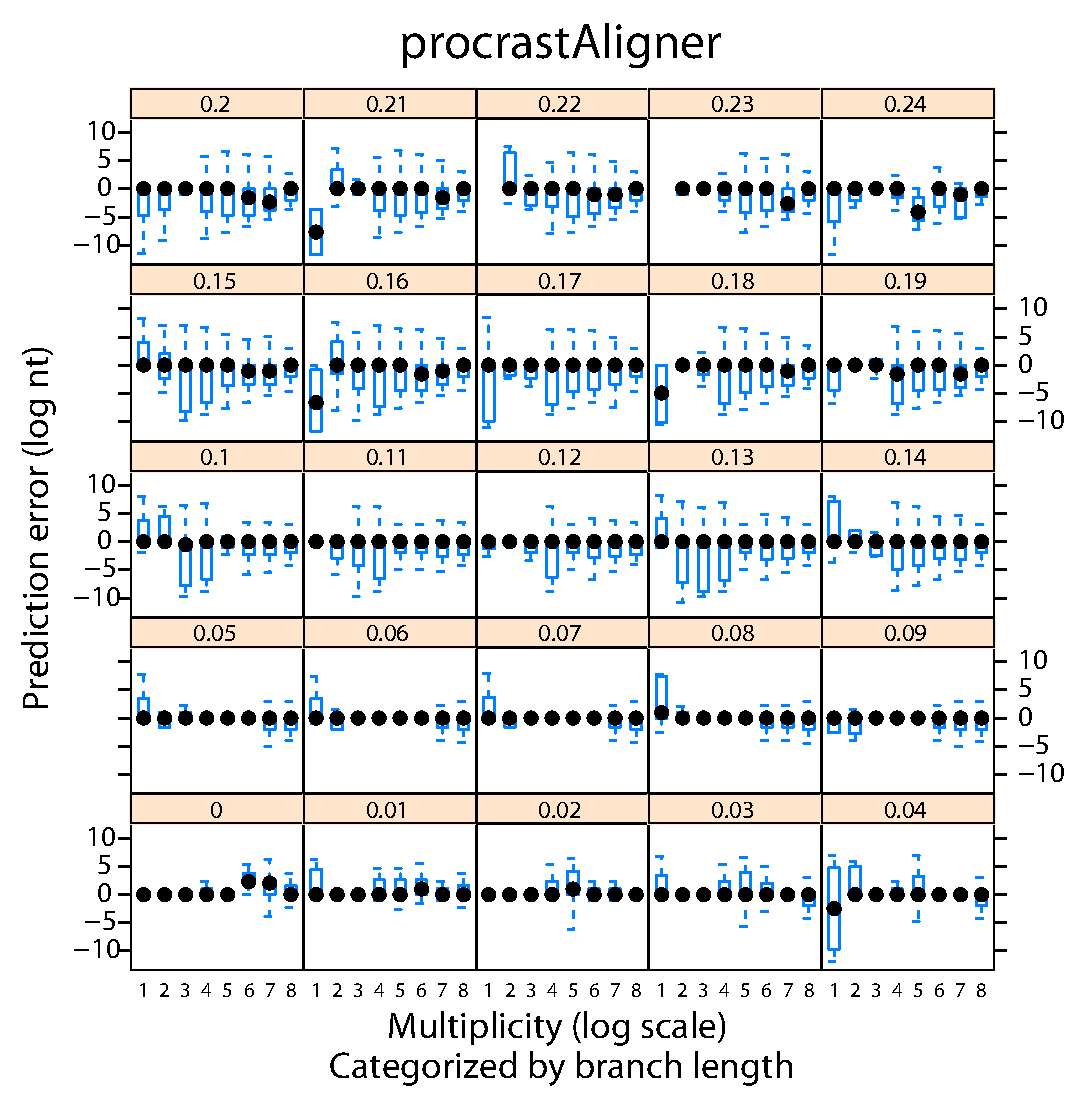
\epsfig{file=./figures/procrast_boundary_fig.eps,width=2.325in}
\label{fig:subfig1}}
\subfigure[]{
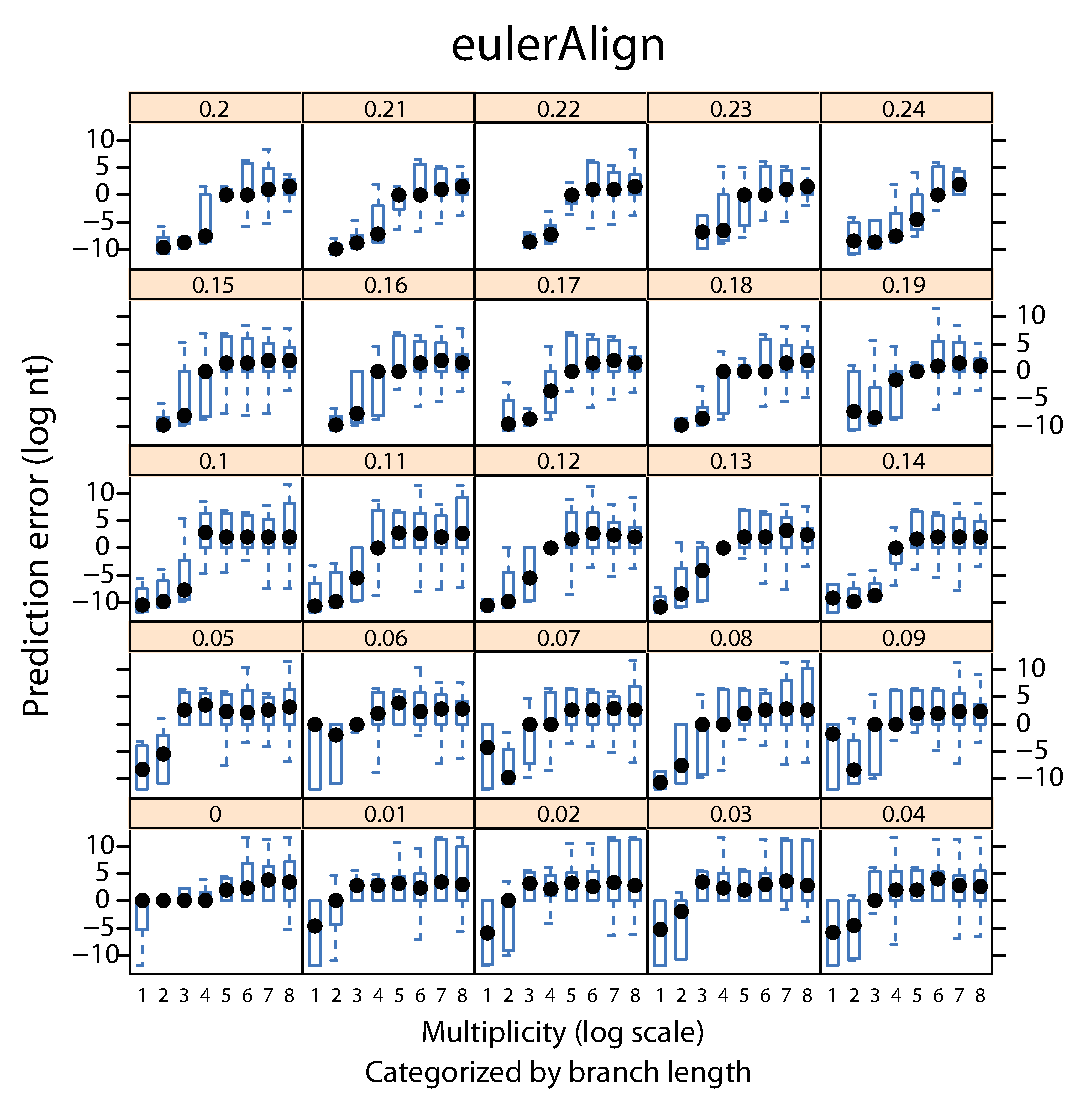
\epsfig{file=./figures/euler_boundary_fig.eps,width=2.325in}
\label{fig:subfig2}}
\caption{\textbf{Boundary prediction performance}. \scriptsize All-pairs boundary prediction accuracy of \texttt{procrastAligner} and \texttt{eulerAlign} were measured for 200 combinations of branch length and multiplicity.  Accuracy on each combination is presented as a box-and-whiskers plot using the scoring metric detailed in Section~\ref{sec:metrics}.  Branch lengths range from 0 to 0.24 and increase by intervals of 0.01.  The $x$-axis label represents the multiplicity of the interspersed repeat in log$_2$-scale. i.e. axis label 8 indicates $2^{8}$ = multiplicity 256. The $y$-axis label is the prediction error in log$_2$-scale nucleotides. Values at 0 represent correctly identified repeat boundaries, values greater than 0 represent overpredictions, and values less than 0 represent underpredictions (see Figure~\ref{fig-overunder}). In general, \texttt{procrastAligner} identifies the true interspersed repeat boundaries more accurately than \texttt{eulerAlign}.}
\label{fig-boundary}
\end{figure}

\section{Discussion}
We have presented a sensitive and efficient gapped-extension heuristic for local
multiple alignment. We have extended our previous results by
converting chains of ungapped multi-matches into gapped local multiple
alignments. Our method is based around an efficient heuristic for
local multiple alignment, featuring a novel method for gapped
extensions joining global multiple alignment with a hidden Markov
model based homology test.  Experimental results demonstrate that the
described method offers a level of alignment accuracy far exceeding
that of previous methods.  Further improvement of the alignment
methodology will likely require increasingly sensitive methods for
seed matching in conjunction with a statistical methodology to assign
significance to local multiple alignments.  One possible avenue to
increase seed matching sensitivity and reduce boundary
underpredictions would be merging overlapping seed matches into a
shorter, higher multiplicity match.  A second avenue would be use of
palindromic seed families instead of using individual seed
patterns. With increased seed matching sensitivity comes additional
false positive seed hits, so a statistical test for rejecting
insignificant local alignments will likely be required.  Exact
computation of $p$-values for local multiple alignments remains a
daunting challenge, although fast approximation methods for pairwise
alignments have shown promise\cite{repseek} and potentially can be
extended to multiple alignments\cite{ref-related1,Prakash2005}.
\begin{figure}[t!]
\centering 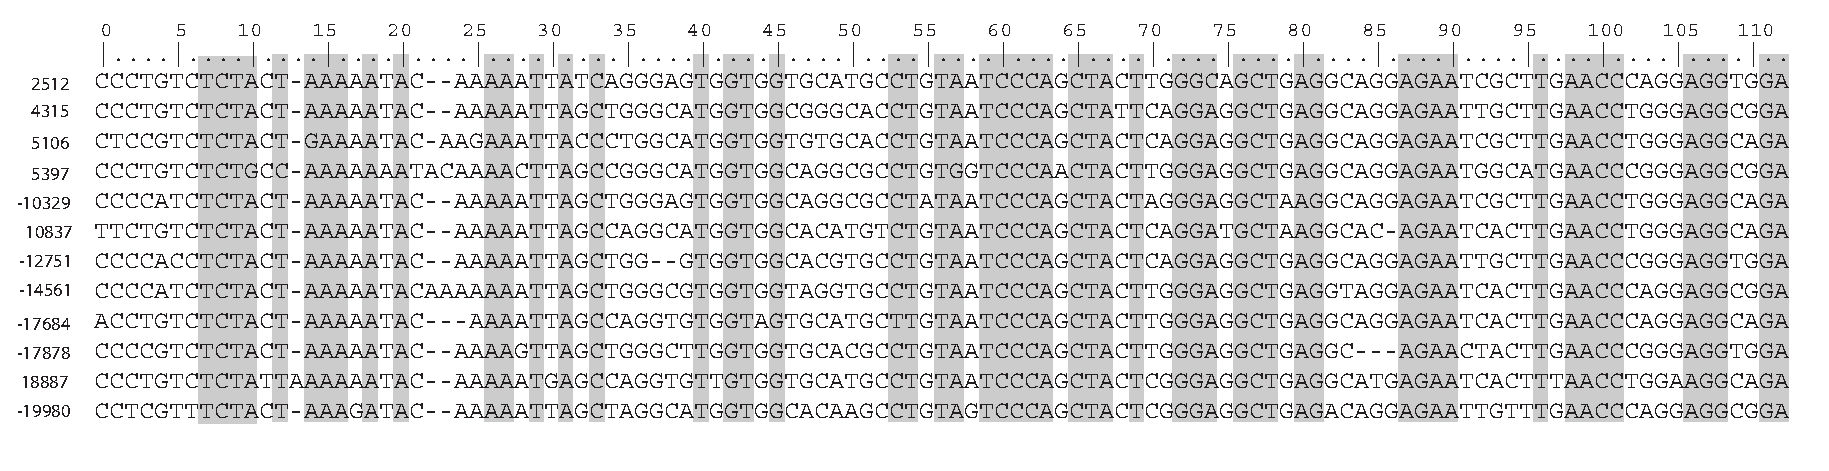
\epsfig{file=./figures/alu_align.eps,width=4.8in}
\vspace{-1.0cm}
\caption{Partial view of an Alu repeat alignment found by procrastAligner in the \emph{H. sapiens} BAC
clone RP11-355H10 (Accession AC010145.10). Each row represents an
aligned Alu. Highlighted columns indicate conserved sequence among all
16 copies of the Alu. Start positions are shown to the left, negative
values indicate complement strand.  Local multiple alignment was
generated with \texttt{procrastAligner} with parameters: \texttt{--z=9
--w=50}.  }
\label{fig-align}
\end{figure}
\subsection{Implementation}
We have implemented our method in a program, \texttt{procrastAligner},
available for Linux, Windows, and Mac OS X. Our open-source
implementation is available as C++ source code licensed under the GPL , and can be downloaded from: \\
\url{http://alggen.lsi.upc.es/recerca/align/procrastination}.

\section{ Acknowledgments }
The authors would like to thank Yu Zhang for providing the
\texttt{eulerAlign} program. We are grateful to Guillaume Achaz for
helpful discussions on the gapped extension algorithm. Accuracy
evaluations utilized a compute resource grant from the Australian
Partnership for Advanced Computing.  AED was supported by NSF grant
DBI-0630765. TJT was supported by Spanish Ministry MECD Grant
TIN2004-03382 and AGAUR Training Grant FI-IQUC-2005.


\bibliographystyle{splncs}
\bibliography{procrastination}

\end{document}
